\documentclass[a4paper,11pt,english]{article}

\usepackage[T1]{fontenc}
\usepackage[utf8]{inputenc}
\usepackage{babel}
\usepackage{lmodern}
\usepackage{inconsolata} % default typewriter kills me
\usepackage{listings}
\usepackage[htt]{hyphenat} % hyphen with tt
\usepackage{enumitem}
\usepackage{fullpage}
\usepackage{graphicx}

\setlist[enumerate]{leftmargin=*}

\setlength{\parindent}{0cm}

\title{COMP --- TP2\\VSL+ Compiler}
\author{Simon Bihel \and Lesly-Ann Daniel}

\begin{document}

\maketitle

\section{Introduction}
The goal of the project was to write a 3address code generator from a AST, built by a provided parser.
The compiler takes a VSL+ program, translates it into 3address code, and returns a MIPS program that can be executed using a Nachos executable.

\section{Work Organization}
\textit{work splitting, code organization, tests}
The tree parser contains 3 files, one main tree parser, one that contains functions to generate three-address code instructions and one file for error detection and handling.
For the development phase, each feature was tested incrementally.
At the beginning we would change the starting rule to test newly added instructions because blocks or functions were not supported yet.

\section{Work Done}
\textit{what has been done}
We added the following VSL+ structures in the suggested order.
\begin{itemize}
 \item simple expressions
 \item affectation
 \item bloc management and scopes
 \item variable management (declaration and use in expressions)
 \item control instructions (if, while and sequence)
 \item definition and function call (with prototypes)
 \item PRINT and READ functions
 \item array management
\end{itemize}

During the compilation, a symbol table with scope handling is inherited and keeps track of the declared structured (functions and variables).
This symbol table is used for error checking.
For each structure, the corresponding errors have been handled in the file \textit{TypeCheck.java}, using the provided \textsc{Error} class.
When a type error is detected, the compilation aborts with an elaborated error message (line, error type, identifiers...).
An example of such error is provided in section \ref{sec.error}.

\section{Tests}
\textit{tests done}
We wrote a bash script that executes our compiler on the provided tests and compares the text output to what is expected, so we can quickly spot errors. An example of execution is provided in section \ref{sec.error}.

We also wrote our own test in \textit{tests/monprogramme.vsl} and \textit{tests/monprogramme2.vsl} which use all the implemented structures.
We encountered a difficulty in the second one when trying to call the function \textsc{plusgrandstrict(t[min], t[i])}.
Indeed, the function call ends up with the wrong values (twice t[i]).
We tried to store \textsc{t[min]} and \textsc{t[i]} in variables and that made the trick (e.g \textit{tests/monprogramme.vsl}).
However we tried to figure out why the first version was not running as expected although the generated 3aCode was correct.
We looked at the generated mips code and noticed that the arguments were stored twice.
We removed the second store as illustrated in section \ref{sec.mips} and the program was running as expected. 

\section{Possible Optimizations}
During a TD class we discussed optimizations that could be implemented in this project by adding an optimization phase in the tree parser.
\begin{itemize}
 \item Decreasing ordering of variables declarations: small size variables are declared first so the padding added for data structure alignment is minimal.
 \item Loop unfolding that would allow to cut out some variables re-declarations.
 \item Checking array access: some compilers add a control structure around array access to ensure that the access is is the array bounds. 
\end{itemize}

\section{Conclusion}
\textit{difficulties encountered, what we've learned, ...}
There was proposed tests for array pointer parameters.
While we were told that we did not have to pass them, interesting questions emerged.
From available types of objects, it does not seem feasible.

\appendix
\section{Example of test execution}
\label{sec.test}
\section{Example of compilation error}
\label{sec.error}
\section{Problem encountered with the generated mips code}
\label{sec.mips}
\begin{figure}[h]
\centering
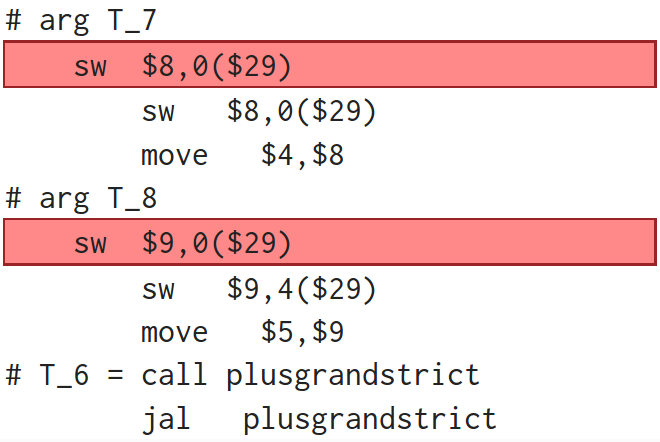
\includegraphics[scale=0.4]{diff}
\caption{
  \textbf{Mips code generated for \textit{tests/monprogramme2.vsl}}.
  The code doesn't work since the first argument is overwritten by the second.
  If the red lines are removed, the program is working.}
\label{prodcons}
\end{figure}


\end{document}
